%%%%%%%%%%%%%%%%%%%%%%%%%%%%%%%%%%%%%%%%%%%%%%%%%%%%%%%%%%%%%%%%%%
%%%%%%%% ICML 2015 EXAMPLE LATEX SUBMISSION FILE %%%%%%%%%%%%%%%%%
%%%%%%%%%%%%%%%%%%%%%%%%%%%%%%%%%%%%%%%%%%%%%%%%%%%%%%%%%%%%%%%%%%

% Use the following line _only_ if you're still using LaTeX 2.09.
%\documentstyle[icml2015,epsf,natbib]{article}
% If you rely on Latex2e packages, like most moden people use this:
\documentclass{article}

% use Times
\usepackage{times}
% For figures
\usepackage{graphicx} % more modern
%\usepackage{epsfig} % less modern
\usepackage{subfigure}

\usepackage{natbib}
\usepackage{amsmath,amsfonts,amscd,amssymb}
\usepackage{dsfont}
\renewcommand{\vec}[1]{\mathbf{#1}}
\usepackage{hyperref}
\DeclareMathOperator*{\argmax}{argmax}
\DeclareMathOperator*{\argmin}{argmin}
\DeclareMathOperator*{\Corr}{Corr}
\newcommand{\R}{\mathds{R}}
\usepackage{multicol}
\usepackage{multirow}
\usepackage{pbox}

% As of 2011, we use the hyperref package to produce hyperlinks in the
% resulting PDF.  If this breaks your system, please commend out the
% following usepackage line and replace \usepackage{icml2015} with
% \usepackage[nohyperref]{icml2015} above.
\usepackage{hyperref}

% Packages hyperref and algorithmic misbehave sometimes.  We can fix
% this with the following command.
\newcommand{\theHalgorithm}{\arabic{algorithm}}

% Employ the following version of the ``usepackage'' statement for
% submitting the draft version of the paper for review.  This will set
% the note in the first column to ``Under review.  Do not distribute.''
\usepackage{icml2015}

% Employ this version of the ``usepackage'' statement after the paper has
% been accepted, when creating the final version.  This will set the
% note in the first column to ``Proceedings of the...''
%\usepackage[accepted]{icml2015}


% The \icmltitle you define below is probably too long as a header.
% Therefore, a short form for the running title is supplied here:
\icmltitlerunning{Automating Political Bias Prediction}

\begin{document}

\twocolumn[
\icmltitle{Automating Political Bias Prediction}

% It is OKAY to include author information, even for blind
% submissions: the style file will automatically remove it for you
% unless you've provided the [accepted] option to the icml2015
% package.
\icmlauthor{Felix Biessmann}{felix.biessmann@gmail.com}
\icmladdress{}
\icmlauthor{Pola Lehmann}{pola.lehmann@wzb.eu}
\icmladdress{Wissenschaftszentrum Berlin}

% You may provide any keywords that you
% find helpful for describing your paper; these are used to populate
% the "keywords" metadata in the PDF but will not be shown in the document
\icmlkeywords{}

\vskip 0.3in
]

\begin{abstract}
Every day media generate large amounts of text. An unbiased view on media reports requires an understanding of the political bias of media content. Assistive technology for estimating the political bias of texts can be helpful in this context. This study proposes a simple statistical learning approach to predict political bias from text. Standard text features extracted from speeches and manifestos of political parties are used to predict political bias in terms of political party affiliation and in terms of political views. Results indicate that political bias can be predicted with above chance accuracy. Mistakes of the model can be interpreted with respect to changes of policies of political actors. Two approaches are presented to make the results more interpretable: a) discriminative text features are related to the political orientation of a party and b) sentiment features of texts are correlated with a measure of political power. Political power appears to be strongly correlated with positive sentiment of a text. To highlight some potential use cases a web application shows how the model can be used for texts for which the political bias is not clear such as news articles.
\end{abstract}

\section{Introduction}
\label{sec:intro}
%
Analysis and classifications of political text is and has been a very important tool to generate political science data (Benoit et al. 2015). Traditionally such classifications are done by experts, who read and label the text of interest.\footnote{See for example the Manifesto Project (Budge et al. 2001; Klingemann et al. 2006), the Comparative Agendas Project or Poltext (Pétry/Duval 2015).} This is, however, a very time consuming task and thus sets various limits to the possible amount of data that a few experts can analyze. The growing field of automated text analysis, that allows the analysis of much more text in less time, is therefore of great interest to political scientists. Additionally automated text analyses allow for a more objective and replicable analysis of political text then human coders could achieve (Benoit et al. 2009)

One area which produces large amounts of text which are of high interest for political scientists is modern media. Standard newspapers, but also new forms as twitter, facebook or blogs produce an ever growing amount of text influencing political debate. These texts can be of interest to political scientist in various analyses. The question we will focus on in this analysis is the potential political bias that can be detected in these sources. In many cases it is obvious which political bias an author has. In other cases some expertise is required to judge the political bias of a text. Keeping an unbiased view on what media report on requires to understand the political bias of texts. Different newspaper outlets are, for example, often ascribed as favoring different positions on the political left-right axis. Data from the European Media Systems Survey show that experts clearly associate different media outlets with specific parties (http://www.mediasystemsineurope.org). However such expert surveys on the political bias of newspapers can normally only give us a very general tendency of a newspaper, they do not distinguish between different journalists or different sections. Assistive technology can help in this context to try and obtain a more unbiased sample of information. It gives us the possibility to get a more nuanced view of the spectrum of political positions favored in important news outlets in a country. In this paper we will test whether it is possible to automatically detect political bias in text and if such a model can be used on different kind of texts. The aim of this study is to provide some empirical evidence indicating that leveraging open data sources automated political bias prediction is possible with above chance accuracy. We will test our model on both in-domain and out-of-domain data. Prediction on out-of-domain data is less precise as on in-domain data, but still generating satisfying results.

In order to validate and explain the predictions of the models three strategies that allow for better interpretations of the models are proposed. First the model misclassifications are related to changes in party policies. Second univariate measures of correlation between text features and party affiliation allow to relate the predictions to the kind of information that political experts use for interpreting texts. Third sentiment analysis is used to investigate whether this aspect of language has discriminatory power.

In the following \autoref{sec:data} gives an overview of the data acquisition and preprocessing methods, \autoref{sec:model} presents the model, training and evaluation procedures; in \autoref{sec:results} the results are discussed and \autoref{sec:conclusion} concludes with some interpretations of the results and future research directions.

\section{Data Sets and Feature Extraction}\label{sec:data}
%
All experiments were run on publicly available data sets of German political texts and standard libraries for processing the text. The following sections describe the details of data acquisition and feature extraction.

\subsection{Data}
Annotated political text data was obtained from two sources: a) the plenary debates held in the German parliament ({\em Bundestag}) and b) all manifesto texts of parties winning seats in the election to the German parliament in the current 18th and the last, 17th, legislative period. 

%For the 18th period we also added the manifesto data of three additional parties that did not win seats but nonetheless played a very important role in the political discourse in the run-up to the election. Wollen wir die einfach rauslassen? Käme ja eh nur in einem kleinen Teil der Analyse vor und macht die Beschreibung an mehreren Stellen kürzer.

\paragraph{Parliament discussion data} Parliament texts are annotated with the respective party label, which we take here as a proxy for political bias. The protocols of plenary debates are available through the website of the German Bundestag\footnote{\url{https://www.bundestag.de/protokolle}}; an open source API was used to query the data in a cleaned and structured format\footnote{\url{https://github.com/bundestag}}. In total 22784 speeches were extracted for the 17th legislative period and 11317 speeches for the 18th period, queried until March 2016.

\paragraph{Party manifesto data}
The party manifesto text was taken from the Manifesto Corpus (add citation). The Corpus is accessible through an publicly available API published by the {\em Manifesto Project} \cite{manifesto}. The data released in this project mainly comprises the complete manifestos of all parties that have won seats at a national election. Each quasi-sentence\footnote{A quasi-sentence has the length of an argument. It is never longer than one sentence.} is annotated with one of 56 policy issue categories. Examples for the policy categories are {\em welfare state expansion, welfare state limitation, democracy, equality}; for a complete list and detailed explanations on how the annotators were instructed see \cite{leftright}. In total the 9 manifestos from the 17th and 18th legislative period have been divided into 29451 quasi-sentences. Each observation has been added with two labels: the party affiliation and the manually assigned policy issue aimed at in each specific statement. 

%The party affiliation was used to evaluate the party evaluation classifiers trained on the parliament speeches. For this purpose the data acquisition was constrained to only those parties that were elected into the parliament. For the analyses based on policy issues all parties were considered, also those three that did not make it into parliament.

The length of each annotated statement in the party manifestos is rather short. The median length is 95 characters or 12 words.\footnote{The longest statement is 522 characters (65 words) long, the 25\%/50\%/75\% percentiles are 63/95/135 characters or 8/12/17 words, respectively.} This can be considered as a very valuable property of the data set, because it allows a fine grained resolution of party manifestos and is a good test for media data, as some data like tweets, facebook texts etc. are often very short, too. However for a classifier (as well as for humans) such short sentences can be rather difficult to classify. Benoit et al. (2015), for example, found in an experiment where experts where differentiating whether specific sentences were dealing with economic or social policy only about 35\% agreement between all expert coders. In the Manifesto Project the human coders therefore do not code these statements separately but within context. In order to obtain less 'noisy' data points from each party -- for the party affiliation task only -- all statements were aggregated into eight policy domains using the 56policy categories from the Manifesto Project. Within the Manifesto Project category scheme each of these belongs to one of seven policy domains. These were used to aggregate the data into the following topics: {\em External Relations, Freedom and Democracy, Political System, Economy, Welfare and Quality of Life, Fabric of Society, Social Groups}. An eight topic is generated for all statements not belonging to any one the 56 policy issues, for a complete list see also \cite{leftright}. Most party manifestos covered all eight topics, some party manifestos in the 17th Bundestag only covered seven.

\subsection{Bag-of-Words Vectorization}\label{sec:bow-vectorization}
First each data set was segmented into semantic units; in the case of the party manifesto data the semantic units were the quasi-sentences associated with one of the 56 policy issues, in the case of parliament discussions this were the speeches. Parliament speeches were often interrupted; in this case each uninterrupted part of a speech was considered a semantic unit. Strings of each semantic unit were tokenised and transformed into bag-of-word vectors as implemented in scikit-learn \cite{scikit-learn}. The general idea of bag-of-words vectors is to simply count occurrences of words (or word sequences, also called {\em n-grams}) for each data point. A data point is usually a document, here it is the semantic units of parliament speeches and manifesto sentences, respectively. The text of each semantic unit is transformed into a vector $\vec{x}\in\mathds{R}^d$ where $d$ is the size of the dictionary; the $w$th entry of $\vec{x}$ contains the (normalized) count of the $w$th word (or sequence of words) in our dictionary. Several options for vectorizing the speeches were tried, including term-frequency-inverse-document-frequency normalisation, n-gram patterns up to size $n=3$ and several cutoffs for discarding too frequent and too infrequent words. All of these hyperparameters were subjected to hyperparameter optimization as explained in \autoref{sec:crossvalidation}.


\section{Classification Model and Training}\label{sec:model}
Bag-of-words feature vectors were used to train a multinomial logistic regression model. Let $y\in\{1,2,\dots,K\}$ be the true  label, where $K$ is the total number of labels and $\vec{W}=[\vec{w}_1,\dots,\vec{w}_K]\in\R^{d\times K}$ is the concatenation of the weight vectors $\vec{w}_k$ associated with the $k$th party then
\begin{eqnarray}\label{eq:logreg_multiclass}
p(y=k|\vec{x},\vec{W}) = &\frac{e^{z_k}}{\sum_{j=1}^K e^{z_j}} \qquad \textrm{with }  z_k=&\vec{w}_k^{\top}\vec{x} \\\nonumber
\end{eqnarray}
The performance of the model was optimized using the classification accuracy, but we also report all other standard measures, precision ($TP / (FP + TP$), recall ($TP / (TP + FN)$) and f1-score ($2\times (Prec. \times Rec) / (Prec + Rec.)$). \\

Three different classification problems were considered:
\begin{enumerate}
\item {\bf Classification of party affiliation} (five class / four class problem)
\item {\bf Classification of government membership} (binary problem)
\item {\bf Classification of policy issues} (56 class problem)
\end{enumerate}

Party affiliation is a five class problem for the 17th legislation period, and a four class problem for the 18th legislation period. The policy issue classification is based on the categories of the Manifesto Project, see \autoref{sec:data} and \cite{leftright}.
For both the party affiliation and the government membership prediction, classifiers were trained on the parliament speeches. For the third problem classifiers were trained only on the manifesto data for which policy issue labels were available.

\subsection{Optimisation of Model Parameters}\label{sec:crossvalidation}
The model pipeline contained a number of  hyperparameters that were optimised using cross-validation.
We first split the training data into a training data set that was used for optimisation of hyperparameters and an held-out test data set for evaluating how well the model performs on in-domain data; wherever possible the generalisation performance of the models was also evaluated on out-of domain data. Hyperparameters were optimised using grid search and 3-fold cross-validation within the training set only: A cross-validation split was made to obtain train/test data for the grid search and for each setting of hyperparameters the entire pipeline was trained and evaluated -- no data from the in-domain evaluation data or the out-of-domain evaluation data were used for hyperparameter optimisation. For the best setting of all hyperparameters the pipeline was trained again on all training data and evaluated on the evaluation data sets. For party affiliation prediction and government membership prediction the training and test set were 90\% and 10\%, respectively, of all data in a given legislative period. Out-of-domain evaluation data were the texts from party manifestos. For the policy issue prediction setting there was no out-of-domain evaluation data, so all labeled manifesto sentences in both legislative periods were split into a training and evaluation set of 90\% (train) and 10\% (evaluation).
% Falls wir die Medien nochreinnehmen, muss das bei out-of-domain auch noch erwähnt werden.

\subsection{Sentiment analysis}\label{sec:sentiment_analysis_methods}
A publicly available key word list was used to extract sentiments \cite{remquahey2010}. A sentiment vector $\vec{s}\in\R^d$ was constructed from the sentiment polarity values in the sentiment dictionary. The sentiment index used for attributing positive or negative sentiment to a text was computed as the cosine similarity between BOW vectors $\vec{x}\in\R^d$ and $\vec{s}$

\begin{align}
\frac{\vec{s}^\top \vec{x}}{\|\vec{s}\|\|\vec{x}\|}
\end{align}

\subsection{Analysis of bag-of-words features}\label{sec:correlations_methods}
While interpretability of linear models is often propagated as one of their main advantages, doing so naively without modelling the noise covariances can lead to wrong conclusions, see e.g. \cite{Zien2009, Haufe2013}; interpreting coefficients of linear models (independent of the regularizer used) implicitly assumes uncorrelated features; this assumption is violated by the text data used in this study. Thus direct interpretation of the model coefficients $\vec{W}$ is problematic. In order to allow for better interpretation of the predictions and to assess which features are discriminative correlation coefficients between each word and the party affiliation label were computed. The words corresponding to the top positive and negative correlations are shown in \autoref{sec:word_party_correlations}.

\section{Results}\label{sec:results}

The following section gives an overview of the results for all political bias prediction tasks. Some interpretations of the results are highlighted and a web application of the models is presented at the end of the section. Because of space restrictions, we will only report results fromt he 17th legislative period here. Results are very similar for the 18th legislative period and can be accessed via github.

\subsection{Predicting political party affiliation}
The evaluation results for the political party affiliation prediction on in-domain data (held-out parliamentary speech text) for the 17th Bundestag are listed in \autoref{tab:results_in-domain}.

When predicting party affiliation on text data from the same domain that was used for training the model, average precision and recall values of above 0.6 are obtained. These results are comparable to those of \cite{Hirst2014} who report a classification accuracy of 0.61 on a five class problem predicting party affiliation in the European parliament; the accuracy for the 17th Bundestag is 0.63, results of the 18th Bundestag are difficult to compare as the number of parties is four and the legislation period is not finished yet.

But as the main purpose of this paper is to generate a model that can be used to predict political bias on new data, like media texts, we are interested in the question if the model also produces satisfying results on out-of-domain data. We are therefore also predicting party affiliation on party manifesto text. For out-of domain data the models yield significantly lower precision and recall values between 0.3 and 0.4 \autoref{tab:results_out-of-domain}. This drop in out of domain prediction accuracy is in line with previous findings \cite{Yu2008}.
A main factor that made the prediction on the out-of-domain prediction task particularly difficult is the short length of the strings to be classified, see also \autoref{sec:data}. In order to investigate whether this low out-of-domain prediction performance was due to the domain difference (parliament speech vs manifesto data) or due to the short length of the data points, the manifesto data was aggregated into the previously described party domains, see \autoref{sec:data}. The topic level results are shown in \autoref{tab:results_topic} and demonstrate that when the texts to be classified are sufficiently long and the word count statistics are sufficiently dense the classification performance on out-of-domain data can - at least in some cases - achieve reliable precision and recall values close to 1.0. This increase is in line with previous findings on the influence of text length on political bias prediction accuracy \cite{Hirst2014}.


\begin{table}[t]
\caption{
\label{tab:results_in-domain}
Classification performance on the party affiliation prediction problem for data from the 17th legislative period on in-domain data. $N$ denotes number of data points in the evaluation set.
}
\begin{center}
\begin{tabular}{lcccc}
    &         precision    &recall &  f1-score  & N  \\
\hline \hline
       cducsu   &    0.62  &    0.81  &    0.70  &     706\\
        fdp    &   0.70   &   0.37  &    0.49    &   331\\
     gruene &      0.59  &    0.40   &   0.48   &    298\\
      linke    &   0.71   &   0.61  &    0.65    &   338\\
        spd   &    0.60   &   0.69  &    0.65   &    606\\
\hline
avg / total &      0.64   &   0.63   &   0.62    &  2279 
%
\end{tabular}
\end{center}
\end{table}

\begin{table}[t]
\caption{
\label{tab:results_out-of-domain}
Classification performance on the party affiliation prediction problem for data from the 17th legislative period on out-of-domain data.  Predictions are done on the {\bf sentence level}.
}
\begin{center}
\begin{tabular}{lcccc}
    &         precision    &recall &  f1-score  & N  \\
\hline \hline
    cducsu    &   0.26   &   0.58   &   0.36    &   2030 \\
    fdp    &   0.38   &   0.28   &   0.33    &   2319 \\
     gruene   &    0.47    &  0.20   &   0.28    &  3747\\
      linke     &  0.30  &    0.47    &  0.37    &   1701\\
        spd     &  0.26  &    0.16   &   0.20    &   2278\\
\hline
avg / total    &   0.35  &    0.31  &    0.30   &   12075\\
%
\end{tabular}
\end{center}

\end{table}

\begin{table}[t]
\caption{
\label{tab:results_topic}
{\bf Topic level classification performance} on the party affiliation prediction problem for data from the evaluation set (manifesto texts) of the 17th legislative period. In contrast to single sentence level predictions (see \autoref{tab:results_17}, \autoref{tab:results_18}, \autoref{tab:confusion} for results and \autoref{sec:data} for topic definitions) the predictions made on topic level are reliable in many cases. Note that all manifesto topics of the green party in the 18th Bundestag are predicted to be from the parties of the governing coalition, CDU/CSU or SPD.}
\begin{center}
\begin{tabular}{lcccc}
& \multicolumn{4}{c}{\bf Party Manifestos} \\
& \multicolumn{4}{c}{\bf 17th Bundestag} \\
    &         precision    &recall &  f1-score  & N  \\
    \hline
        \hline
cducsu     &  0.64  &    1.00  &    0.78    &     7\\
       fdp    &   1.00    &  1.00    &  1.00    &     7\\
    gruene  &     1.00  &    0.86  &    0.92    &     7\\
     linke    &   1.00   &   1.00     & 1.00    &     7\\
       spd   &    0.80   &   0.50    &  0.62     &    8\\
    \hline
    avg / total  &     0.88   &   0.86   &   0.86  &      36\\
\end{tabular}
\end{center}

\end{table}

\subsection{Validation}
\paragraph{Differentiability of policy issues}
One reason why some statements are difficult to classify could be that some issues are more difficult to differentiate than others. To test this a separate suite of experiments was run to train and test the prediction performance of the text classifiers models described in \autoref{sec:model}. As there was no out-of-domain evaluation set available in this setting only the evaluation error on in-domain data is reported. Note however that in this experiment too the evaluation data was never seen by any model during training time.
In \autoref{tab:results_avg_political_view} results for the best and worst classes, in terms of predictability, are listed along with the average performance metrics on all classes.
Precision and recall values of close to 0.5 on average can be considered rather high considering the large number of labels. Results are not surprising, but are equal to those by human coders. \\

\begin{table}
\caption{
\label{tab:results_avg_political_view}
Classification of 56 political views, see \autoref{sec:data}.
}
\begin{center}
\footnotesize
\begin{tabular}{lcrrrr}
code & meaning  &      prec    &recall & N\\
\hline\hline
%
       501  & environmentalism + &      0.62   &   0.61 &      165\\
        202 &   democracy + &   0.58  &    0.55   &      122\\
        701    & labour +&  0.57  &    0.54   &   129\\
                201    &freedom/human rights +  & 0.58   &   0.54   &      159\\
         106   & peace + & 0.52&      0.57   &       21\\
\dots\\
        302     &centralism + & 0.25     & 0.20  &          10\\
        401    &  free enterprise + &0.20    &  0.19    &       52\\
        505    &welfare - &  0.13   &   0.14   &      14\\
        409    & keynesian demand +&  0.14  &      0.13   &      8\\
            0    & undefined &  0.09  &    0.12   &    17\\
            \hline
avg / total  &  &  0.47    &  0.46 &    2946\\
%
\end{tabular}
\end{center}
\end{table}

\paragraph{Policy change}
Another explanation for missclassification could lie in the fact that parties change their policy positions. In order to investigate this confusion matrices were extracted for the predictions on the out-of-domain evaluation data for sentence level predictions (see \autoref{tab:confusion}) as well as topic level predictions (see \autoref{tab:confusion_topic}). On the topic level results for the 17th legislative period are pretty good except for the SPD. In the 18th legislative period predictions are very bad for the Green party. One explanation for this missclassification could lie in policy changes. For example, the Green party has devoted large parts of its manifesto to renewable and against nuclear energy. After Fukushima the other parties adopted these positions. \\

% Die könnten wir vielleicht rausnehmen.
% Confusion matrix sentence level
\begin{table}[t]\label{tab:conf_mat_four_class}
\caption{\label{tab:confusion} {\bf Confusion matrices (sentence level)} for predictions on evaluation data (party manifestos); classifiers were trained on parliament speeches for the 17th legislative period; the most prominent effect is the high likelihood for a party to be taken as the strongest, governing party, cdu/csu. This can be interpreted as a change in policies of the conservative party cdu/csu towards the policies of the green party.}
\begin{tabular}{lccccccc}
 \multicolumn{8}{c}{\bf Party Manifestos}\\
 \multicolumn{8}{c}{\bf 17th Bundestag}\\
 \\
&&& \multicolumn{5}{c}{Predicted}\\
&&& cducsu & fdp& gruene& linke& spd\\
\hline
\multirow{5}{*}{\rotatebox{90}{\pbox{3cm}{\centering True}}}& &cducsu &1186 &289& 178& 198& 179\\
&&fdp &882& 658& 236& 329& 214\\
&&gruene &1174& 404& 764& 941& 464\\
&&linke &388& 92& 214& 806& 201\\
&&spd &999& 268& 240& 398& 373\\
\end{tabular}
\end{table}


% Confusion matrix topic level
\begin{table}[t]\label{tab:conf_mat_four_class}
\caption{\label{tab:confusion_topic} {\bf Confusion matrices (topic level)} for predictions on evaluation data (party manifestos) for classifiers trained on parliament speeches for the 17th legislative period (left) and 18th legislative period (right).}
\begin{tabular}{lccccccc}
 \multicolumn{8}{c}{\bf Party Manifestos}\\
 \multicolumn{8}{c}{\bf 17th Bundestag}\\
 \\
&&& \multicolumn{5}{c}{Predicted}\\
&&& cducsu & fdp& gruene& linke& spd\\
\hline
\multirow{5}{*}{\rotatebox{90}{\pbox{3cm}{\centering True}}} &&cducsu &7& 0& 0& 0& 0\\
&&fdp&0& 7& 0& 0& 0\\
&&gruene&0& 0& 6& 0& 1\\
&&linke&0& 0& 0& 7& 0\\
&&spd&4& 0& 0& 0& 4\\
\end{tabular}
\end{table}


\begin{table*}[t]
\caption{
\label{tab:results_binary_17}
Classification performance on the binary prediction problem in the 17th legislative period, categorizing speeches into government (FDP/CDU/CSU) and opposition (Linke, Gr\"une, SPD).
}
\begin{center}
\begin{tabular}{lcccccccc}
& \multicolumn{4}{c}{\bf Held-out parliament speeches} & \multicolumn{4}{c}{\bf Party Manifestos}\\
    &         precision    &recall &  f1-score  & N    &         precision    &recall &  f1-score  & N\\
\hline \hline
government    &   0.83   &   0.84&      0.84     & 1037 & 0.49  &    0.59 &     0.54  &    4349\\
 opposition     &  0.86  &    0.86   &   0.86    &  1242 & 0.74 &     0.66  &    0.70   &   7726\\
\hline
avg / total   &    0.85 &     0.85 &     0.85  &    2279 & 0.65  &     0.63  &     0.64  &    12075\\

%
\end{tabular}
\end{center}
\end{table*}

\begin{table*}[t]
\caption{
\label{tab:results_binary_18}
Classification performance on the binary prediction problem in the 18th legislative period, categorizing speeches into government (SDP/CDU/CSU) and opposition (Linke, Gr\"une).
}
\begin{center}
\begin{tabular}{lcccccccc}
& \multicolumn{4}{c}{\bf Held-out parliament speeches} & \multicolumn{4}{c}{\bf Party Manifestos}\\
    &         precision    &recall &  f1-score  & N    &         precision    &recall &  f1-score  & N\\
\hline \hline
government   &    0.88  &    0.95    &  0.92   &    786   &0.52   &   0.66 &     0.58  &    5972\\
 opposition    &   0.86    &  0.71   &   0.78   &    346 & 0.69  &    0.56    &  0.62   &   8229\\
\hline
avg / total    &   0.88    &  0.88     & 0.87  &    1132 &  0.62   &   0.60    &  0.60 &    14201\\
%
\end{tabular}
\end{center}
\end{table*}

%
%\subsection{Correlations between words and parties}\label{sec:word_party_correlations}
%We now know that party affiliation can be predicted using our model. But which words are most important for the classification performed here? To get a more precise idea of what differentiates the parties from each other the 10 highest and lowest correlations between individual words and the party affiliation label are shown for each party in \autoref{fig:party_word_correlations}. Correlations were computed on the data from the current, 18th, legislative period. Some unspecific stopwords are excluded.
%The following paragraphs highlight some examples of words that appear to be preferentially used or avoided by each respective party. Even though interpretations of these results are problematic in that they neglect the context in which these words were mentioned some interesting patterns can be found and related to the actual policies the parties are promoting.
%% Vielleicht sollten wir hier dann auch Beispiel aus der 17 nehmen.
%\paragraph{\bf Left party (linke)}
%The Left party talks mainly about issues related to work ({\em Besch\"aftigten}) and unemployment ({\em Hartz IV, Erwerbslosen}). 
%\paragraph{\bf Green party (gruene)}
%The Green party talks about the formal procedures available to opposition parties to question government policy ({\em fragen, anfragen}) and, interestingly, about the reform of the Germany army ({\em R\"ustungsprojekte, Wehrbericht}).
%\paragraph{\bf Social Democratic Party (SPD)}
%The SPD often uses words related to rights of the working class ({\em International Labour Organisation, Arbeitnehmerrechte}) and the governing coalition ({\em bundestagsfraktion, koalitionspartner}).
%
%\paragraph{\bf Christian Democratic Union/Christian Social Union (CDU/CSU)}
%The CDU/CSU party often uses words related to a pro-economy attitude, such as competitiveness or (economic) development ({\em Wettbewerbsf\"ahigkeit, Entwicklung}) and words related to security ({\em Sicherheit}). 
%
%\begin{figure}
%\begin{center}
%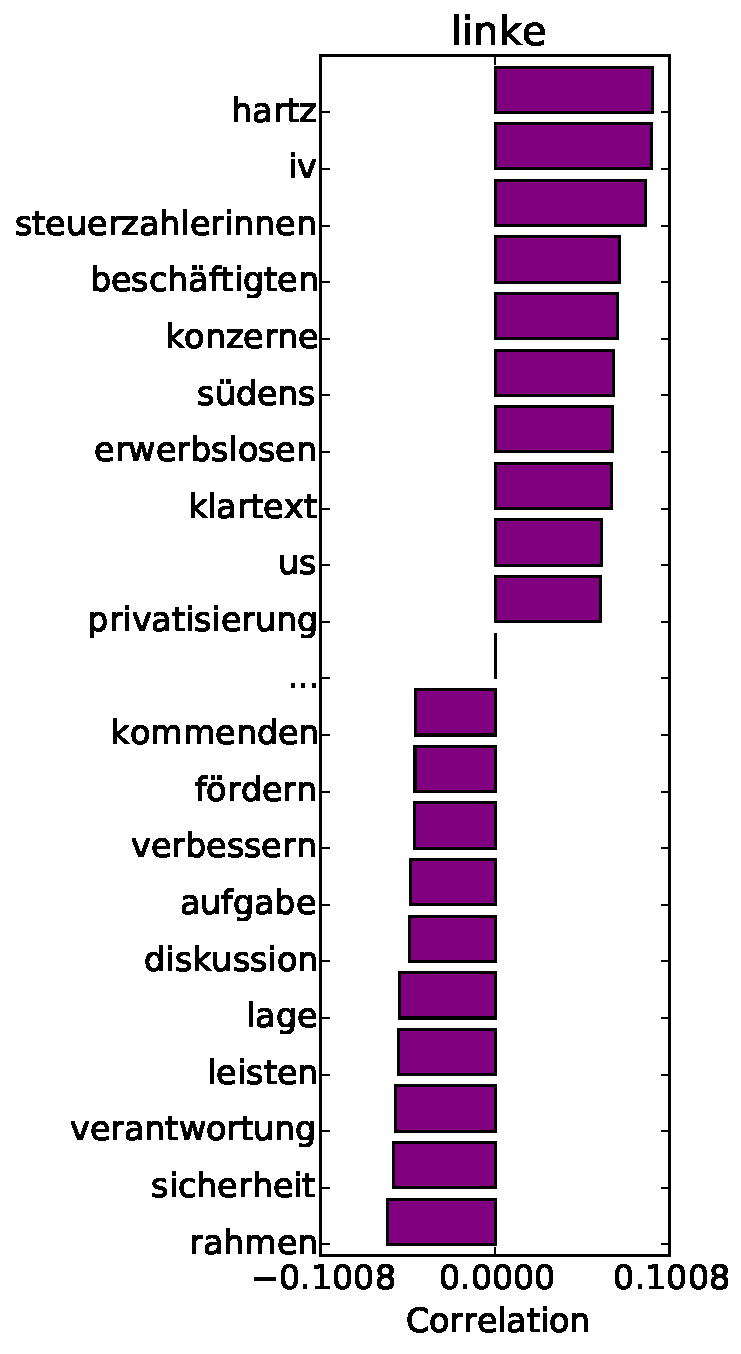
\includegraphics[width=2.8cm]{images/party_word_correlations-linke-18.pdf}
%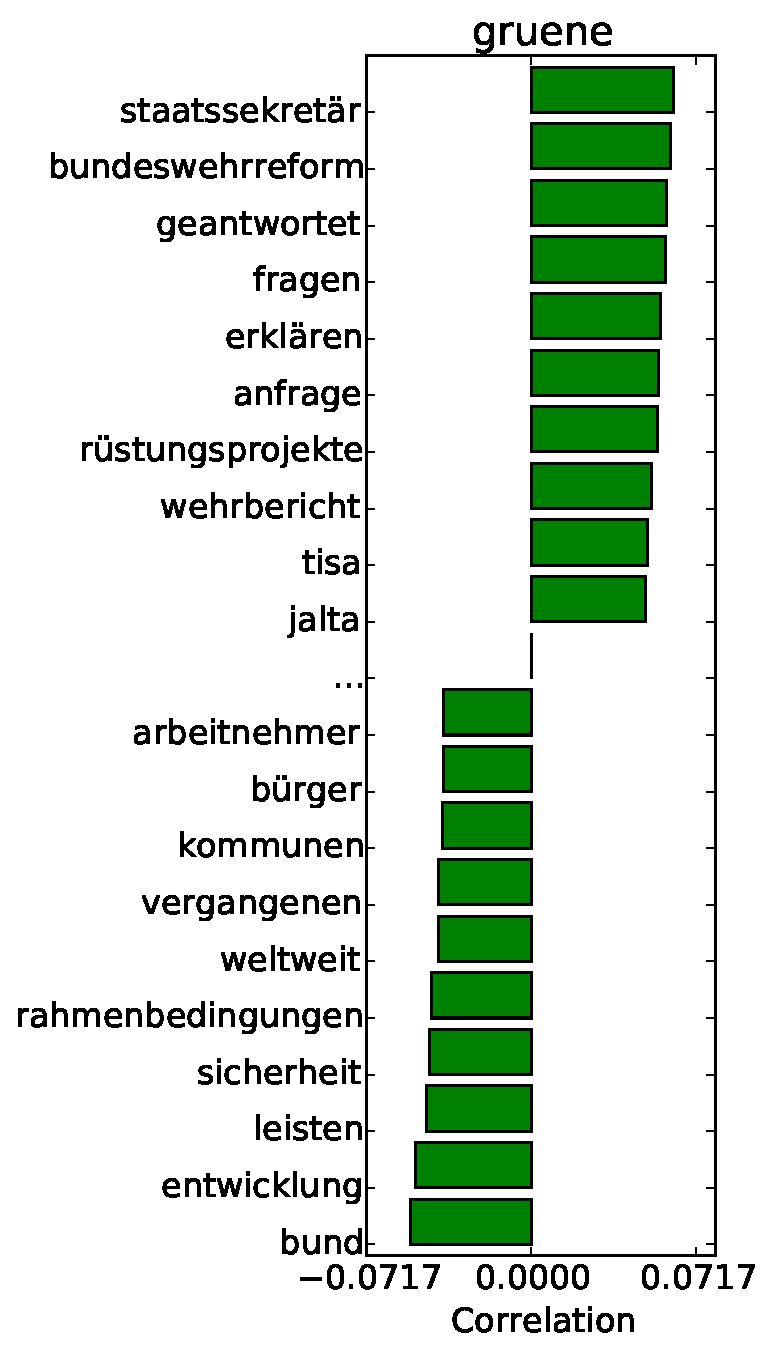
\includegraphics[width=2.9cm]{images/party_word_correlations-gruene-18.pdf}
%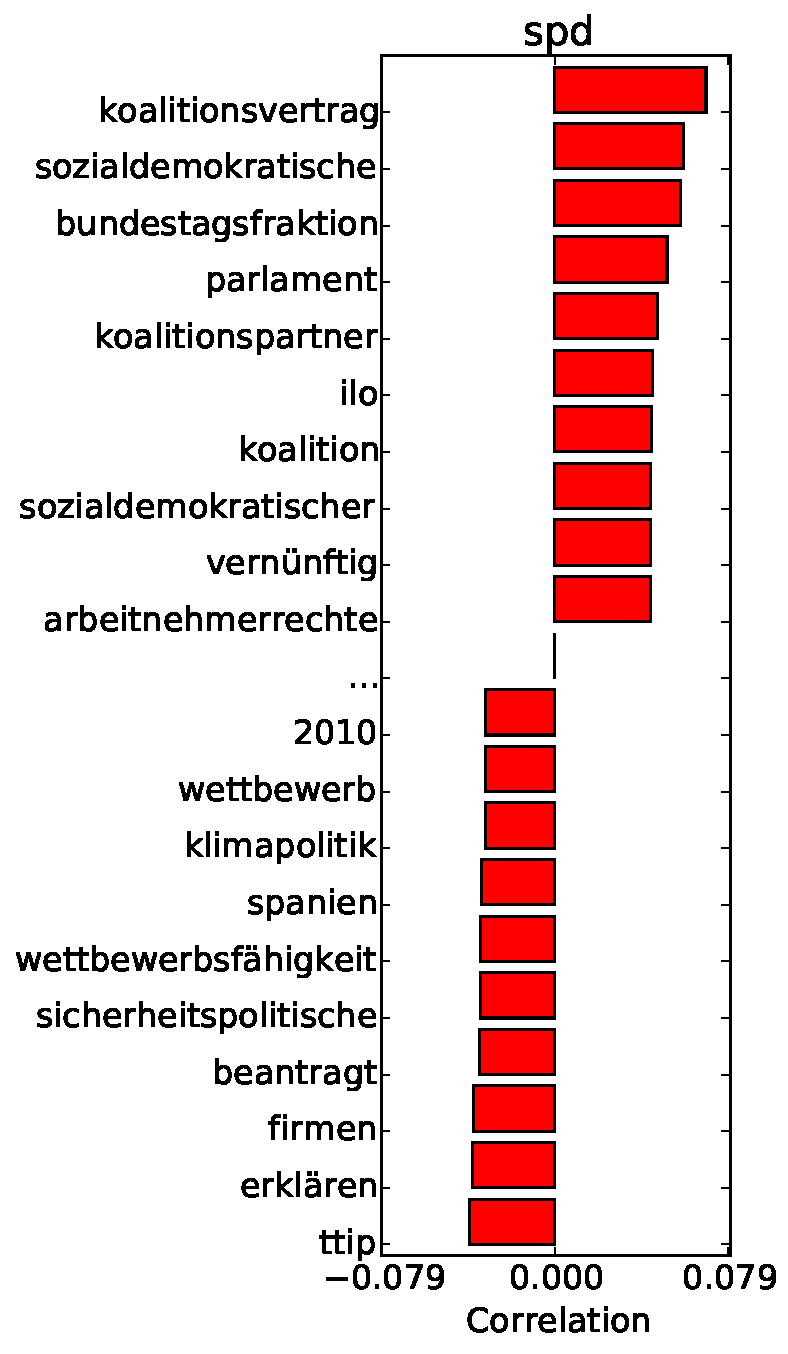
\includegraphics[width=3cm]{images/party_word_correlations-spd-18.pdf}
%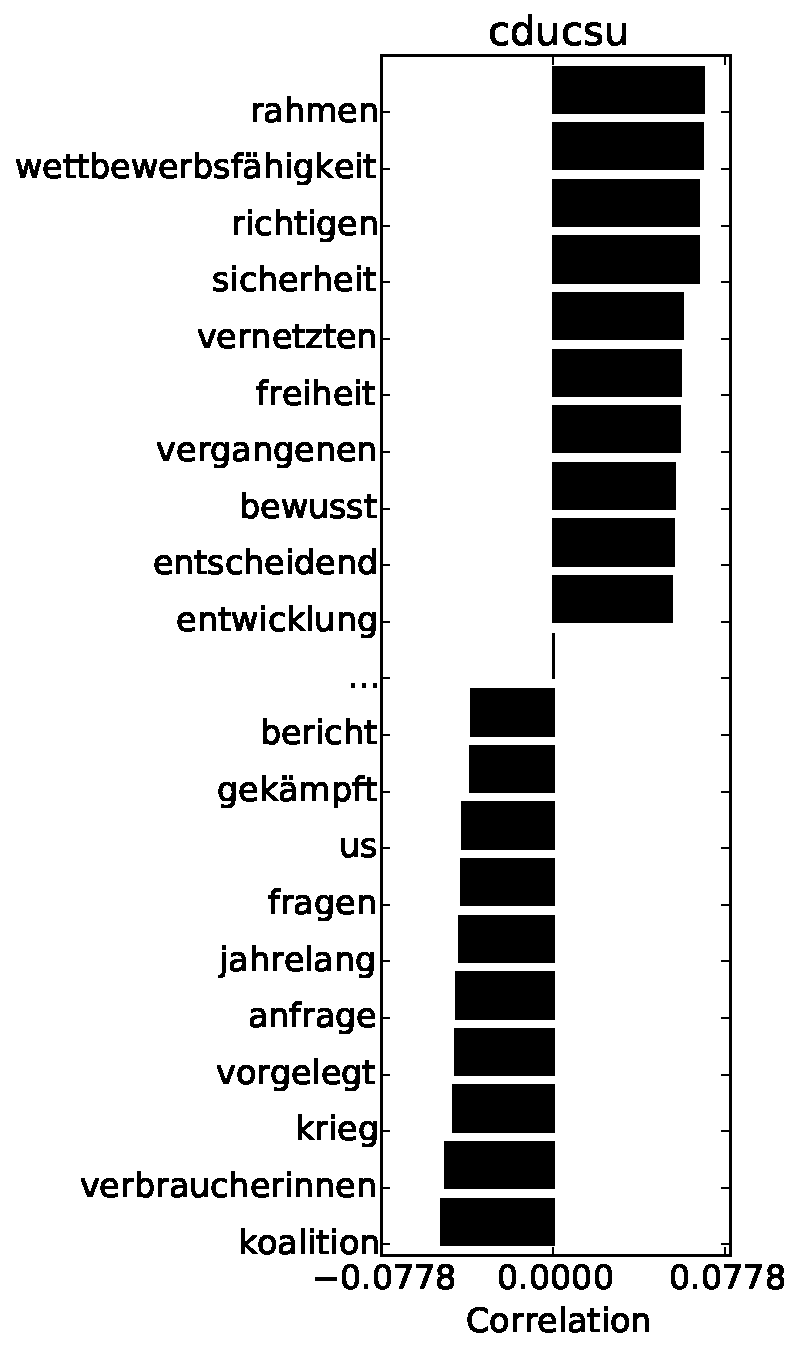
\includegraphics[width=3cm]{images/party_word_correlations-cducsu-18.pdf}
%%
%\end{center}
%\caption{
%\label{fig:party_word_correlations}
%Correlations between words and party affiliation label for parliament speeches can help interpreting the features used by a predictive model. Shown are the top 10 positively and negatively correlated text features for the current Bundestag. For interpretations see \autoref{sec:word_party_correlations}.}
%\end{figure}


\subsection{Predicting government status}\label{sec:sentiment_result}
Next to the party affiliation labels also government membership labels were used to train models that predict whether or not a text is from a party that belonged to a governing coalition of the Bundestag. In \autoref{tab:results_binary_17} the results are shown for the 17th legislative period. While the in-domain evaluation precision and recall values reach values close to 0.9, the out-of-domain evaluation drops again to values between 0.6 and 0.7. This is in line with the results on binary classification of political bias in the Canadian parliament \cite{Yu2008}. The authors report classification accuracies between 0.8 and 0.87, the accuracy in the 17th Bundestag was 0.85. While topic-level predictions were not performed in this binary setting, the party affiliation results in \autoref{tab:results_topic} suggest that a similar increase in out-of-domain prediction accuracy could be achieved when aggregating texts to longer segments. \\


\paragraph{Speech sentiment correlates with political power} 
But what are the underlying features that give rise to the classifiers performance? In order to investigate this the bag-of-words features were analysed with respect to their sentiment. The average sentiment of each political party is shown in \autoref{fig:party_sentiments}. High values indicate more pronounced usage of positive words, whereas negative values indicate more pronounced usage of words associated with negative emotional content.

The results show an interesting relationship between political power and sentiment. Political power was evaluated in terms of membership of the government. Correlating these indicators of political power with the mean sentiment of a party shows a strong positive correlation between speech sentiment and political power. This pattern is evident from the data in \autoref{fig:party_sentiments} and in \autoref{tab:sentiments}: In the current Bundestag, government membership correlates with positive sentiment with a correlation coefficient of 0.98 and the number of seats correlates with 0.89.

Note that there is one party, the social democrats (SPD), which has many seats and switched from opposition to government with the 18th Bundestag: With its participation in the government the average sentiment of this party switched sign from negative to positive, suggesting that positive sentiment is a strong indicator of government membership.


\begin{figure}
\begin{center}
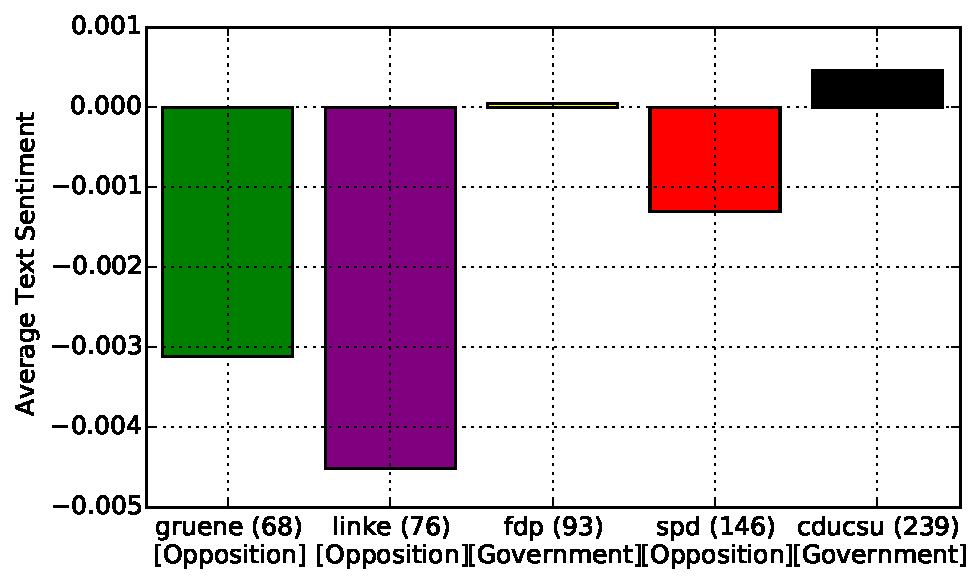
\includegraphics[width=6cm]{images/party-sentiments-17.pdf}  \hfill 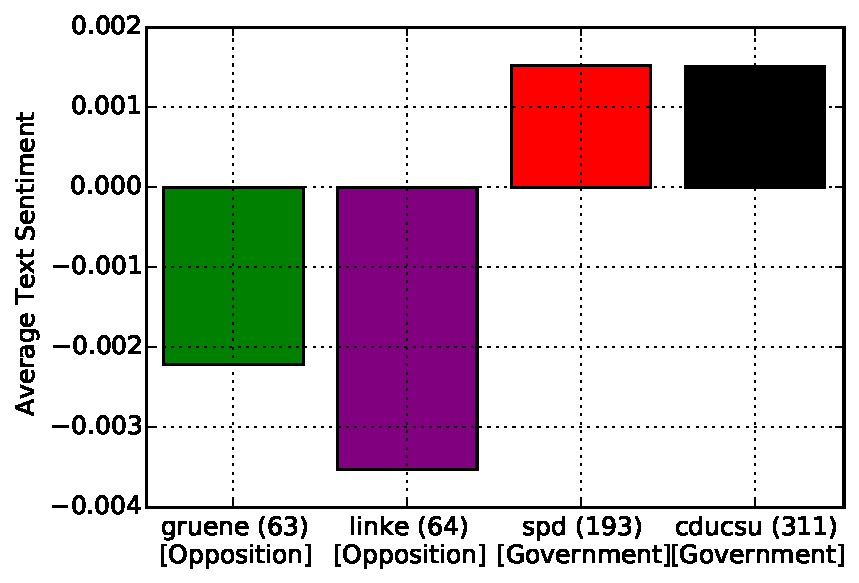
\includegraphics[width=5cm]{images/party-sentiments-18.pdf}
%
\end{center}
\caption{
\label{fig:party_sentiments}
Speech sentiments computed for speeches of each party; parties are ordered according to the number of seats in the parliament. There is a trend for more positive speech content with more political power. Note that the SPD (red) switched from opposition to government in the 18th Bundestag: their seats in the parliament increased and the average sentiment of their speeches switched sign from negative to overall positive sentiment.
}
\end{figure}

\begin{table}[t]
\caption{
\label{tab:sentiments}
Correlation coefficient between average sentiment of political speeches of a party in the german Bundestag with two indicators of political power, a) membership in the government and b) the number of seats a party occupies in the parliament.
}
\begin{center}
\begin{tabular}{lcc}
   Sentiment vs. &          Gov. Member    &  Seats\\
\hline\hline
17th Bundestag    &  0.84 & 0.70\\
18th Bundestag   &  0.98 & 0.89\\
%
\end{tabular}
\end{center}
\end{table}




\subsection{An example web application}
To show an example use case of the above models a web application was implemented that downloads regularly all articles from some major German news paper websites\footnote{\url{http://www.spiegel.de/politik}, \url{http://www.faz.net/aktuell/politik}, \url{http://www.welt.de/politik}, \url{http://www.sueddeutsche.de/politik}, \url{http://www.zeit.de/politik}} and applies some simple topic modelling to them. For each news article topic, headlines of articles are plotted along with the predictions of the policy issue of an article and two labels derived deterministically from the 56 class output, a left right index and the political domain of a text, see \cite{leftright}. Within each topic it is then possible to get an ordered (from left to right) overview of the articles on that topic. An example of one topic that emerged on March 31st is shown in \autoref{fig:fipi}. A preliminary demo is live at \cite{fipidemo} and the code is available on github\cite{fipi}.
\begin{figure}
\begin{center}
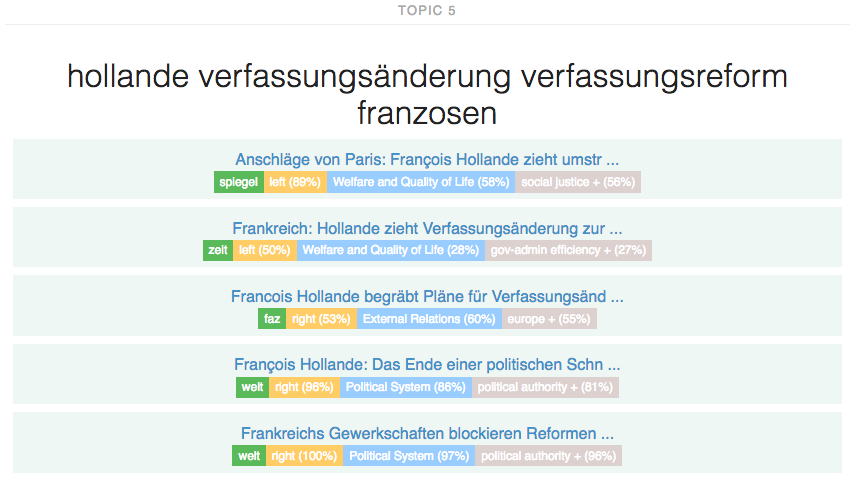
\includegraphics[width=10cm]{images/fipi-screenshot}
%
\end{center}
\caption{
\label{fig:fipi}
A screen shot of an example web application using the political view prediction combined with topic modelling to provide a heterogeneous overview of a topic. }
\end{figure}


\section{Conclusions, Limitations and Outlook}\label{sec:conclusion}
This study presents a simple approach for automated political bias prediction. The results of these experiments show that automated political bias prediction is possible with above chance accuracy in some cases. It is worth noting that even if the accuracies are not perfect, they are above chance and comparable with results of comparable studies \cite{Yu2008, Hirst2014}. While these results do not allow for usage in production systems for classification, it is well possible to use such a system as assistive technology for human annotators in an active learning setting.

One of the main limiting factors of an automated political bias prediction system is the availability of training data. Most training data sets that are publicly available have an inherent bias as they are sampled from a different domain. This study tried to quantify the impact of this effect.
For the cases in which evaluation data from two domains was available there was a pronounced drop in prediction accuracy between the in domain evaluation set and the out of domain evaluation set. This effect was reported previously for similar data, see e.g. \cite{Yu2008}. Also the finding that shorter texts are more difficult to classify than longer texts is in line with previous studies \cite{Hirst2014}. When considering texts of sufficient length (for instance by aggregating all texts of a given political topic) classification performance improved and in some cases reliable predictions could be obtained even beyond the training text domain.

Some aspects of these analyses could be interesting for social science researchers; three of these are highlighted here.
First the misclassifications of a model can be related to the changes in policy of a party. Such analyses could be helpful to quantitatively investigate a change in policy. Second analysing the word-party correlations shows that some discriminative words can be related to the political views of a party; this allows for validation of the models by human experts. Third when correlating the sentiment of a speech with measures of political power there is a strong positive correlation between political power and positive sentiment. While such an insight in itself might seem not very surprising this quantifiable link between power and sentiment could be useful nonetheless: Sentiment analysis is a rather domain independent measure, it can be easily automated and scaled up to massive amounts of text data. Combining sentiment features with other measures of political bias could potentially help to alleviate some of the domain-adaptation problems encountered when applying models trained on parliament data to data from other domains. \\


All data sets used in this study were publicly available, all code for experiments and the live web application can be found online \cite{fipi, fipidemo}.

\subsection*{Acknowledgements}
We would like to thank Friedrich Lindenberg for factoring out the \url{https://github.com/bundestag/plpr-scraper} from his Bundestag project. Some backend configurations for the web application were taken from an earlier collaboration with Daniel Kirsch. Michael Gaebler provided helpful feedback on an earlier version of the manuscript. 
%
\small{
\bibliographystyle{plain}
\bibliography{political_bias_prediction}
}


\end{document}


% This document was modified from the file originally made available by
% Pat Langley and Andrea Danyluk for ICML-2K. This version was
% created by Lise Getoor and Tobias Scheffer, it was slightly modified
% from the 2010 version by Thorsten Joachims & Johannes Fuernkranz,
% slightly modified from the 2009 version by Kiri Wagstaff and
% Sam Roweis's 2008 version, which is slightly modified from
% Prasad Tadepalli's 2007 version which is a lightly
% changed version of the previous year's version by Andrew Moore,
% which was in turn edited from those of Kristian Kersting and
% Codrina Lauth. Alex Smola contributed to the algorithmic style files.
